\documentclass[a4paper,12pt]{article}
\usepackage[utf8]{inputenc}
\usepackage{amsmath, amssymb, amsthm, graphicx, pgfplots}
\usepackage{lmodern}
\pgfplotsset{compat=1.18}

\title{Fourier-Methoden: Theorie und Anwendungen}
\author{Felix Wager}
\date{\today}

\begin{document}

\maketitle

\renewcommand{\contentsname}{Inhaltsverzeichnis}
\tableofcontents
\newpage

\section{Abstract}

\section{Einleitung}
\subsection{Motivation}
Warum Fourier-Methoden heute so wichtig sind.
\subsection{Zielsetzung der Arbeit}
\subsection{Aufbau der Arbeit}

\section{Mathematische Grundlagen}
\subsection{Historischer Hintergrund}
Fourier und Wärmeleitung.
\subsection{Komplexe Zahlen und die Eulerformel}
Um sich die Arbeit mit Fourier Transformationen, Reihen und sonstigem erheblich zu erleichtern ist es sehr sinnvoll mit komplexen Zahlen zu arbeiten. Doch was sind komplexe Zahlen? 
Komplexe Zahlen sind prinzipiell nichts anderes, als eine Erweiterung der Menge der Reellen Zahlen, welche es ermöglicht die Wurzel von negativen Zahlen zu ziehen. Dafür wird die Wurzel die imaginäre Einheit $i$ definiert. Mathematisch korrekt sieht das wie folgt aus:
$$i^2 = -1$$
Die Menge der komplexen Zahlen wird mit dem Symbol $\mathbb{C}$ abgekürzt. Eine typische komplexe Zahl hat in der algebraischen Schreibweise die Form:
$$ z = a + ib \quad \text{mit} \quad a,b \in \mathbb{R} $$
$a$ ist hierbei der Realteil $\Re(z)$ und $b$ der Imaginärteil $\Im(z)$ von $z$. \vspace{1em}

Um mit komplexen Zahlen bei Fourier Reihen zu arbeiten, benötigt man auch ein paar Rechenoperationen. Die wichtigsten beiden sind hier der Betrag und das komplex konjugierte einer komplexen Zahl. Eine komplexe Zahl lässt sich auch als Vektor im $\mathbb{R}^2$ betrachtet, so ist dann der Betrag als euklidische Norm dieses Vektors definiert. 
$$\vert{z}\vert = \sqrt{ a^2 + b^2}$$
Bedeutet in einem Koordinatensystem, bei dem der Real- und Imaginärteil einer Zahl auf den x- und y-Achsen festgehalten wird, ist der Betrag die Länge vom Ursprung bis zum Punkt im Koordinatensystem dieser Zahl. 
Und das komplex konjugierte einer Zahl ist eine Abbildung, welche lediglich den Imaginärteil mit $-1$ multipliziert:

$$\bar{}\;:\mathbb{C}\;\to\mathbb{C},\; z = x+iy \mapsto \bar{z} := x-iy$$

Mithilfe von komplexen Zahlen und den Taylorreihen von Sinus, Cosinus und der Exponentialfunktion $e^x$ kann man nun die Eulerformel herleiten. 

% $$e^{ix} = \cos{x} + i\sin{x}$$

Wenn man den Betrag dieses Ausdrucks bildet, so fällt auf, dass hier das Ergebnis, unabhängig von $x$, 1 ist. Dies bedeutet, dass $e^{ix}$ als ein gegen den Uhrzeigersinn rotierender Vektor, für steigende Werte für $x$, gesehen werden kann. Im vorher genannten Koordinatensystem, welches man auch die Gaußsche Zahlenebene nennt, sieht das so aus:
\begin{center}
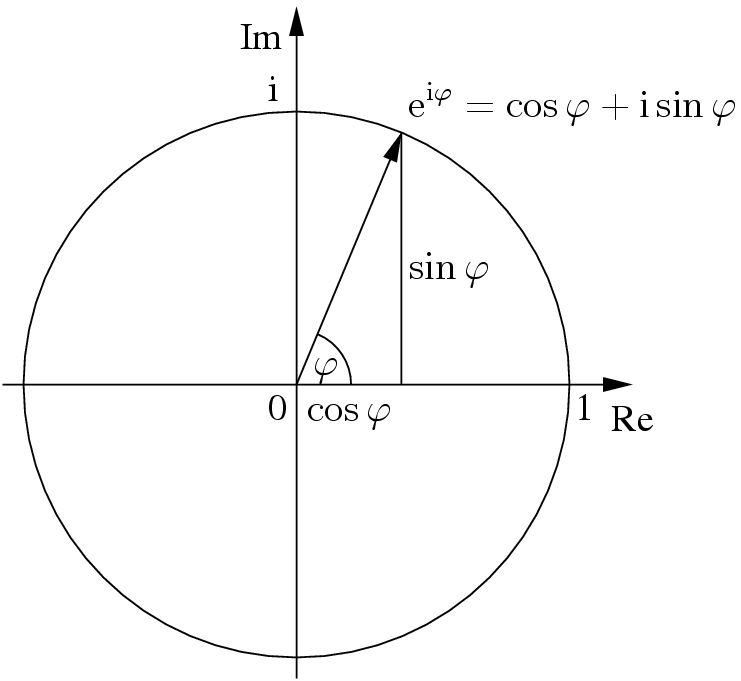
\includegraphics[scale=0.75]{eulerformel.jpg}
\end{center}

\subsection{Skalarprodukt von Funktionen und Orthonormalsysteme}

\section{Fourier-Reihe}
\subsection{Herleitung der Reihe}
\subsection{Berechnung der Koeffizienten}
\subsection{Eigenschaften und Konvergenz}

\section{Von der Reihe zur Fourier-Transformation}
\subsection{Übergang zum Integral}
\subsection{Fourier-Transformation und inverse Transformation}
\subsection{Eigenschaften}
Linearität, Verschiebung, Faltung.

\section{Diskrete Fourier-Transformation (DFT)}
\subsection{Definition und Motivation}
\subsection{Herleitung aus der Fourier-Transformation}
Eigene Herleitung
\subsection{Beweise für die Korrektheit}
\subsection{FFT als effiziente Berechnung}

\section{Eigene Beiträge}
\subsection{Eigene Herleitung der DFT}
\subsection{Beweise}
\subsection{Eigener FFT-Algorithmus in Python}
\subsection{Audio-Programm zur Echtzeit-Visualisierung}

\begin{figure}[h!]
\centering
\begin{tikzpicture}
\begin{axis}[
    width=\textwidth,
    height=8cm,
    xlabel={Zeit [s]},
    ylabel={Zeit [s]},
    grid=major,
    major grid style={gray!30},
    legend style={at={(0.5,-0.2)}, anchor=north, legend columns=2, font=\small},
    label style={font=\large},
    tick label style={font=\small},
    line width=1pt,
    no markers,
    cycle list={
        {blue},
        {red},
        {brown},
        {black},
        {teal}
    }
]

\addplot table[x index=1, y expr=\thisrowno{2}/1000] {fft_bench5.dat};
\addlegendentry{Rekursive FFT}

\addplot table[x index=1, y expr=\thisrowno{3}/1000] {fft_bench5.dat};
\addlegendentry{Iterative FFT}

\addplot table[x index=1, y expr=\thisrowno{4}/1000] {fft_bench5.dat};
\addlegendentry{Iterative FFT auf GPU}

\addplot table[x index=1, y expr=\thisrowno{5}/1000] {fft_bench5.dat};
\addlegendentry{cuFFT-Bibliothek (GPU)}

\addplot table[x index=1, y expr=\thisrowno{6}/1000] {fft_bench5.dat};
\addlegendentry{FFTW-Bibliothek (CPU)}


\end{axis}
\end{tikzpicture}
\caption{Vergleich der FFT-Methoden anhand der Benchmarks.}
\end{figure}

\begin{figure}[h!]
\centering
\begin{tikzpicture}
\begin{axis}[
    width=\textwidth,
    height=8cm,
    xlabel={Zeit [ms]},
    ylabel={Zeit [ms]},
    grid=major,
    major grid style={gray!30},
    legend style={at={(0.5,-0.2)}, anchor=north, legend columns=2, font=\small},
    label style={font=\large},
    tick label style={font=\small},
    line width=1pt,
    no markers,
    cycle list={
        {blue},
        {red},
        {brown},
        {black},
        {teal}
    }
]

\addplot table[x expr=\thisrowno{1}*1000, y index=2] {fft_bench_small.dat};
\addlegendentry{Rekursive FFT}

\addplot table[x expr=\thisrowno{1}*1000, y index=3] {fft_bench_small.dat};
\addlegendentry{Iterative FFT}

\addplot table[x expr=\thisrowno{1}*1000, y index=4] {fft_bench_small.dat};
\addlegendentry{Iterative FFT auf GPU}

\end{axis}
\end{tikzpicture}
\caption{Vergleich der FFT-Methoden für die zweite Messreihe.}
\end{figure}

\begin{figure}[h!]
\centering
\begin{tikzpicture}
\begin{axis}[
    width=\textwidth,
    height=8cm,
    xlabel={Zeit [min]},
    ylabel={Zeit [s]},
    grid=major,
    major grid style={gray!30},
    legend style={at={(0.5,-0.2)}, anchor=north, legend columns=2, font=\small},
    label style={font=\large},
    tick label style={font=\small},
    line width=1pt,
    no markers,
    cycle list={
        {black},
        {teal}
    }
]

\addplot table[x expr=\thisrowno{1}/60, y expr=\thisrowno{2}/1000] {fft_bench_big.dat};
\addlegendentry{cuFFT-Bibliothek (GPU)}

\addplot table[x expr=\thisrowno{1}/60, y expr=\thisrowno{3}/1000] {fft_bench_big.dat};
\addlegendentry{FFTW-Bibliothek (CPU)}

\end{axis}
\end{tikzpicture}
\caption{Vergleich der FFT-Methoden für die zweite Messreihe.}
\end{figure}

\subsection{Bildverarbeitung: Moiré-Muster entfernen mit 2D-FFT}

\section{Anwendungen}
\subsection{Audio}
Echtzeitaufnahme und Visualisierung, Tonhöhenerkennung oder Noise Cancelling, Ergebnisse.
\subsection{Bild}
Röntgenbild und Moiré-Filterung, Ergebnisse.

\section{Diskussion}
\subsection{Bewertung der Ergebnisse}
\subsection{Stärken und Grenzen}
\subsection{Bedeutung im größeren Kontext}

\section{Fazit und Ausblick}
\subsection{Zusammenfassung der Ergebnisse}
\subsection{Ausblick: Erweiterungen und Anwendungen}

\end{document}
